%%%%%%%%%%%%%%%%%%%%%%%%%%%%%%%%%%%%%%%%%%%%%%%%%%%%
%%%%%%%%%%%%%%%%% Code Validation %%%%%%%%%%%%%%%%%%
%%%%%%%%%%%%%%%%%%%%%%%%%%%%%%%%%%%%%%%%%%%%%%%%%%%%


\section{\textit{aztekas} code validation}
\label{sec:codevalid}

In order to validate \textit{aztekas} for its research usage, in this section we present a number of numerical tests and comparison with analytic solutions in the non-relativistic regime. All simulations presented here were computed using a second order Runge-Kutta method. The specific flux calculation, Courant number, primitive variable reconstruction and recovery, will be specified at each test.

\begin{table}
    \centering
    \caption{Initial parameters for the four tests of the 1D shock tube problem. The labels $L$ and $R$ represent the initial left and right states, respectively.}
    \begin{tabular}{c|cccc}
    \hline 
    Parameters & Test 1 & Test 2 & Test 3 & Test 4  \\
    \hline 
    $\rho_L$ & 1.0   & 10.0  & 1.0  & 5.0 \\
    $p_L$    & 1.0   & 13.33 & 0.2  & 1.0 \\
    $v_L$    & 0.0   & 0.0   & -1.5 & 0.5 \\
    $\rho_R$ & 0.125 & 1.0   & 1.0  & 1.0 \\
    $p_R$    & 0.1   & 0.01  & 0.2  & 1.0 \\
    $v_R$    & 0.0   & 0.0   & 1.5  & 0.0 \\
    $\gamma$ & 5/3   & 5/3   & 5/3  & 1.4 \\
    \hline
    \end{tabular}
    \label{tab:sod}
\end{table}

%%%%%%%%%%%%%%% Shock Tube %%%%%%%%%%%%%%%%%

\subsection{Shock tube}
\label{subsec:sod}

\subsubsection{One dimensional shock tube}
\label{subsubsec:shock}

The shock tube test, first presented by~\citet{sod1978}, consists on a Riemann problem along the entire integration domain. The 1D problem has an exact solution which is presented, for the non-relativistic case, by~\citet{toro2009}. This test has also been performed with \textit{aztekas} using the PVRS discretization~\eqref{eq:pvrs} in the relativistic regime~\citep[see][]{aguayo2018}.

The numerical solution was computed for various test, changing the initial density, pressure and velocity. All the results presented for the Shock tube test use the HLLE formula, a MC limiter for the linear reconstruction of the primitive variables, a domain [0,1] with $N = 400$ identical cells, and a Courant number of 0.9. The initial discontinuity is placed at $x = 0.5$. Unless it is specified, all simulations where performed using the classical primitive variable recovery, this is, $\mathbf{u}$ is recover directly from $\mathbf{q}$.

\begin{figure}
    \centering
    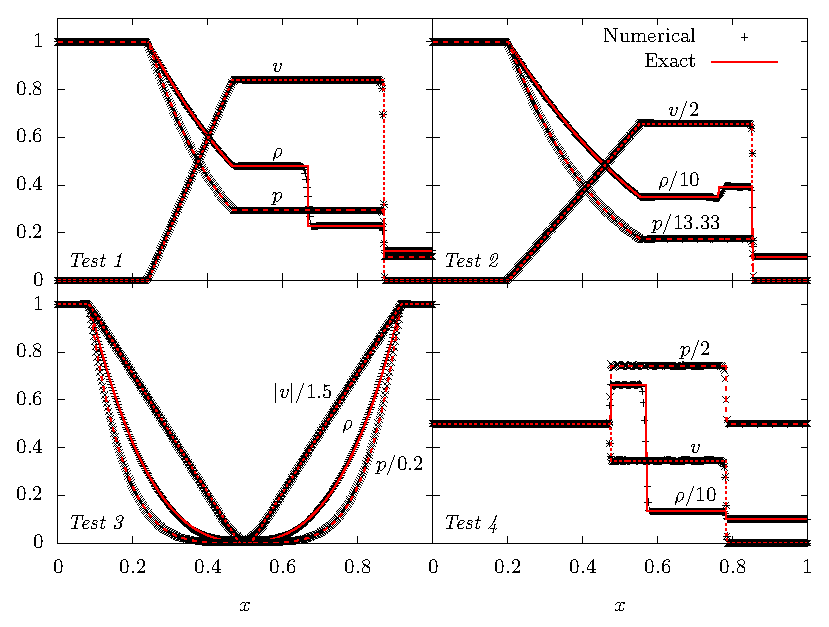
\includegraphics[width=0.47\textwidth]{Figures/sodtests.eps}
    \caption{Results of the 1D shock tube tests for the four sets of initial conditions listed in Table~\ref{tab:sod}. Each panel corresponds to a different test and compares the density, pressure and velocity as obtained against their corresponding analytic values. In all cases t=0.2.}
    \label{fig:sodtests}
\end{figure}

\begin{figure}
    \centering
    \includegraphics[width=0.47\textwidth]{Figures/lnorm.eps}
    \caption{$L^1-$norm of the error in the density versus the resolution $N$ for all tests presented in Table~\ref{tab:sod}. In a dotted line, for comparison, we present the slope that a first order of convergence must have.}
    \label{fig:lnorm}
\end{figure}


In Table~\ref{tab:sod} we show the initial parameters for the left ($x < 0.5$) and right ($x > 0.5$) state of the shock tube problem. These tests were selected in order to obtain different kind of intermediate states. In Test 1 and 2 two different type of working surface with a rarefaction wave are created, in Test 3 two rarefaction waves induces a lower density zone and in Test 4 a strong shock without a rarefaction wave is formed. The boundary conditions wer set as free outflow in both directions by copying the value of the last evolved cell onto the adjacent ghost cells (zero order extrapolation).

%with a rarefaction wave were created (Test 1 and 2), two rarefaction waves induces a lower density zone (Test 3) and were a strong shock without rarefaction wave is formed (Test 4). The boundary conditions were set as outflow in both directions, and this was computed by doing a zero order extrapolation to the ghost cells, i.e., by setting the value of the last valid control volume to all ghost cells.ex

In Figure~\ref{fig:sodtests} we show the density, pressure and velocity at a time $t=0.2$ for the four tests. The figure shows the results of the numerical simulations compared against the corresponding exact, analytic values~ \citep{toro2009}. As can be seen from this figure, for all cases there is a good agreement between the numerical and the analytic solutions all over the domain.

In order to determine the convergence rate of the code, we repeated the same four tests presented in Table~\ref{tab:sod}, using six different resolutions $N_1 = 100$, $N_2 = 200$, $N_3 = 400$, $N_4 = 800$, $N_5 = 1600$ and $N_6 = 3200$. We compute the $L_1$ norm of the error between the numerical and the analytical solution. The order of convergence $Q$ is estimated as 
\begin{equation}
Q \approx \frac{\log(e_{i+1}/e_i)}{\log(\Delta x_{i+1}/\Delta x_i)},
\end{equation}

\noindent where $e_i$ is the $i$-th error obtained for the $\Delta x_i$ resolution. The result is shown in Figure~\ref{fig:lnorm} and, as expected due to the presence of discontinuities (see Section~\ref{subsubsec:riemann_solver}), the order of convergence is $\sim 1$ for all tests, due to the presence of discontinuities.

%%%%%%%%% Shock tube - Cyl and Sph %%%%%%%%%%

\subsubsection{Shock tube test in cylindrical and spherical coordinates}
\label{subsubsec:sodcylsph}

\begin{figure}
    \centering
    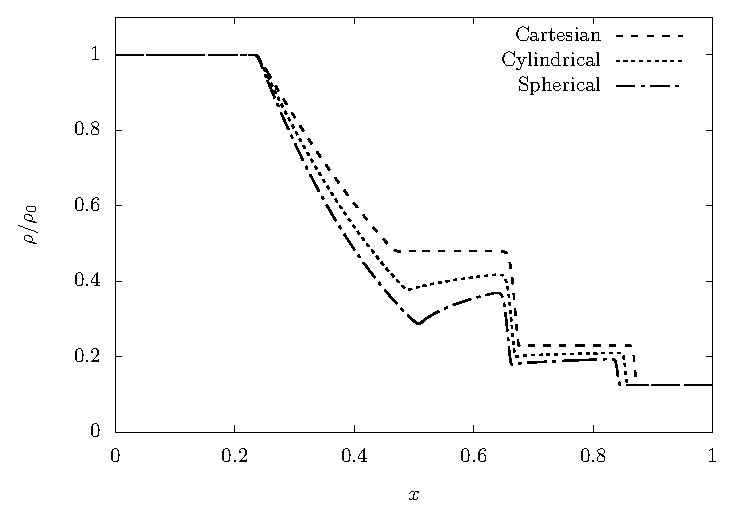
\includegraphics[width=0.47\textwidth]{Figures/comb.eps}
    \caption{Comparison of the density profile in Cartesian, cylindrical and spherical coordinates for the Test 1 in Table~\ref{tab:sod}.}
    \label{fig:comp}
\end{figure}

In addition to Cartesian coordinates, we have also implemented within \textit{aztekas} the use of cylindrical and spherical coordinate systems. In this Subsection, we present the results of the 1D shock tube test for these geometries. This kind of tests have been done presented by other authors~\citep[e.g.][]{radice2012,lora2015}, although it is not commonly considered as part of a test suite because as a numerical suited test because there are not analytic solutions to this problem in spherical and cylindrical geometries. All simulations for this case were done with a HLLE flux calculator, the MC reconstruction, the standard primitive variable recovery and a grid of $N=400$ points.

In Figure~\ref{fig:comp} we show the results of the density in this test for the spherical and cylindrical versions of Test 1 in Table~\ref{tab:sod} at $t=0.2$. For comparison, we also show in this figure the result obtained with Cartesian coordinates discussed in the previous Subsection. As can be seen, due to geometrical source terms in the balanced equations (see Appendix~\ref{A:cylsph}), the form of the density profile differs in all cases. 
%In particular, 1D spherical simulations are really useful for problems with a complete spherical symmetry, as would be seen below with the spherical accretion tests.


%%%%%%% Multidim - Shock Tube %%%%%%%%%

\subsubsection{Two dimensional shock tube}
\label{subsubsec:2dsod}

\begin{figure}
    \centering
    \includegraphics[width=0.47\textwidth]{Figures/shock-d.png}
    \caption{Density profile of an initial configuration of Test 1 with an interface located at $x + y = 1$ at time $t = 0.2$.}
    \label{fig:diag}
\end{figure}
\begin{figure}
    \centering
    \includegraphics[width=0.47\textwidth]{Figures/diag.eps}
    \caption{Density, pressure and velocity profile along the diagonal $x=y$, compared with the exact solution.}
    \label{fig:diag-1d}
\end{figure}

We performed the shock tube problem for one of the tests of Table~\ref{tab:sod} along a diagonal in a $400 \times 400$ cartesian grid in order to analyze the flux calculation along two dimensions simultaneously.~\citep[see][were a similar study was implemented for the relativistic case]{lora2015}.

\begin{figure*}
    \centering
    \includegraphics[width=0.95\textwidth]{Figures/reflection.png}
    \caption{Isocontour density plot of the double mach reflection at a time $t=0.25$.}
    \label{fig:reflection}
\end{figure*}

In Figure~\ref{fig:diag} we show the snapshot of the shock tube evolution at time $t=0.2$ for the Test 1 of Table~\ref{tab:sod}. We use the HLLC flux formula, the MC limiter and the standard primitive variable recovery. The left and right states were delimited by a line with equation $x + y = 1$. The boundary conditions were set as outflow in all directions. For this case we implemented a linear extrapolation to the ghost cells in the boundaries in order to avoid spurious reflections. Although, as can be seen from Figure~\ref{fig:diag}, the solution still shows a problem in the boundaries, specifically at the bottom-right and upper-left corners, where a small diminishing in the density is observed. It is likely that this is because the extrapolation was done independently for each direction. In Figure~\ref{fig:diag-1d} we show the density, pressure and velocity profile along the diagonal $x=y$, and compare the numerical results against the analytic solution.


\subsection{Double Mach reflection}
\label{subsec:strongshock}

The HRSC methods are designed not only for the accurate resolution of the position and sharpness of discontinuities, like shock waves, but also to avoid spurious numerical instabilities, as the \textit{carbuncle instability}~\citep{rodionov2018}\footnote{Some authors~\citep[e.g.]{moschetta2001} claim that, rather to be a numerical pathology, the carbuncle instability is intrinsically associated to the Euler equations.}. This instability appears when a shock wave interacts with other shocks or reflecting walls, and manifests as a growing protuberance ahead of the discontinuity. This spurious problem seems to appear when a less dissipative method is used in the simulation~\citep{woodward1984}.

The double Mach reflection test was first described by~\citet[][]{woodward1984}, and it is part of some codes test suite~\citep[e.g.]{stone2008}. The problem consists on a strong shock wave moving diagonally toward a reflecting wall.
Although there is not analytic solution for this problem, is a commonly used problem for testing that shocks propagate at the correct speed in all directions (avoid the carbuncle instability) and the proper reflective boundaries implementation.

In order to test the stability of the solution, this test was performed using the WENO5 reconstructor and the HLLC flux calculator, which is a less dissipative method (compare with the HLLE). We also performed a high resolution simulation on a Cartesian domain $[0,4]\times[0,1]$, with $1200\times300$ uniformly distributed grid cells. We use a polytropic index $\gamma = 1.4$, the standard primitive variable recovery and a Courant number of 0.5.

Our initial and boundary conditions closely follows those by~\citet{stone2008}. The domain was divided into a pre-shock and post-shock region, delimited by a discontinuity that forms a 60$^\circ$ angle with the $x$-axis, intersecting it at $x_0 = 1/6$. The shock zone moves diagonally towards the lower boundary with a Mach number of 10, so the initial conditions are

 \begin{equation}
     \left( \rho, p \right) = \left\lbrace
     \begin{array}{cl}
        (8,116.5) & \mathrm{if}\, x < x_0 + y/\sqrt{3} \\
        (1.4,1) &   \mathrm{if}\, x \geq x_0 + y/\sqrt{3},
     \end{array}
     \right.
 \end{equation}
 
\noindent with velocity components for the post-shock zone
\begin{equation}
    \begin{split}
        v_x &= 8.5 \cos(30^\circ), \\
        v_y &= -8.5 \sin(30^\circ),
    \end{split}
\end{equation}

\noindent and the pre-shock zone initially at rest.

We set free outflow conditions at the left and right boundaries and reflection at the lower boundary for $x > x_0$. For $x < x_0$ we fill the ghost cells with the values of the post-shock zone. For the upper boundary, we impose the ghost cells to follow the movement of the diagonal shock, so we set the pre-shock conditions for $x \geq x_s(t)$ and the post-shock conditions for $x < x_s(t)$ where
\begin{equation}
    x_s(t) = x_0 + \frac{1 + 20t}{\sqrt{3}},
\end{equation}

\noindent is the position of the shock at the upper boundary. This initial conditions were taken from~\citet{woodward1984}.

In Figure~\ref{fig:reflection} we show the density contour levels of the double mach reflection for a time $t = 0.25$. This result is in good agreement with the one presented in other works~\citep[e.g.][]{she2016}: the contact surface curly jet, that appears along reflecting wall, does not reach the shock front, avoiding the carbuncle instability. 





%%%%%%%%%%%%% Sedov %%%%%%%%%%%%%%%%

\subsection{Sedov blast wave}
\label{subsec:sedov}

The Sedov blast wave~\citep{sedov1959} consists of an intense explosion caused by an enormous amount of energy deposited in a small volume at the center of the domain, which generates a strong spherically symmetric shock which propagates through a homogeneous medium.

This problem was studied by~\citet{sedov1959}, finding a self-similar solution evolves in time as the shock front radius is given by~\citep{sedov1959,landau1987}:
\begin{equation}
    r(t) = \left( \frac{E_0}{\alpha \rho_0} \right)^{1/5} t^{2/5},
    \label{eq:self-sim-sedov}
\end{equation}

\begin{figure}
    \centering
    \includegraphics[width=0.47\textwidth]{Figures/sedov.eps}
    \caption{Comparison between numerical results and the analytic solution of the density, pressure and velocity  for the 2D spherical axisymmetric simulation of the Sedov blast wave. We only plot the profiles along $\theta = \pi/4$ as no angular dependence was shown.}
    \label{fig:sedov}
\end{figure}

\noindent where $E_0$ is the initial energy injected, $\rho_0$ is the background density and $\alpha$ is a constant that depends on the equation of state. This solution is relevant in astrophysics as it helps to understand the physics behind a supernovae explosion. The Sedov blast wave is a commonly used benchmark test for hydrodynamic codes~\citep{tasker2008}.

Continuing with the 2D tests, for this simulation we implement a 2D spherically axisymmetric grid with $400 \times 20$ cells uniformly distributed over a $[0,8]\times[0,\pi/2]$ domain. We use the HLLC flux calculator, the MC reconstructor and a Courant number of 0.25, as well as the standard primitive variable recovery. We set an initial explosion energy of $E_0 = 1.25 \times 10^5$ inside a radius $r_0$ that corresponds to 8 numerical cells near the origin. The initial pressure $p_0$ was computed using the polytropic EoS as
\begin{equation}
    p_0 = \frac{3(\gamma - 1) E_0}{4 \pi \rho_0 r_0^3},
\end{equation}

\noindent were the polytropic index was set to $\gamma = 5/3$. The gas is set initially at rest and $\rho_0 = 1$. The explosion shock front propagates through a static medium with $p_m = 0.00001$ and $\rho_m = \rho_0$. We use free outflow conditions at both inner and outer radial boundaries and reflection along the axis $\theta = 0$ and $\pi/2$.

In Figure~\ref{fig:sedov} we show the density, pressure and velocity profiles of the Sedov explosion at $t=0.1$ along the $\theta = pi/4$ direction. For comparison, we also show the corresponding analytic solution~\citet{kamm2000}. As can be seen, there is a good agreement between the numerical results and the analytic solution, the shock is well resolved, as expected for the HLLC Riemann solver.

In order to determine the convergence rate for this test, we repeated the simulation using different radial resolutions, maintaining the same number of cells along $\theta$. We compute the $L^1-$norm using the standard primitive variable recovery and the PVRS discretization~\eqref{eq:pvrs}. In Figure~\ref{fig:lnorm-sedov}, we show that, for both methods, the order of convergence is $~1$, which is expected due to the strong shock front. For a higher resolution, the convergence rate decreases in both cases, this is the result of the truncation error being dominated by the rounding error\footnote{The truncation error is the difference between the exact solution and a numerical solution obtained with certain method. The rounding error is due to the precision of the computer~\citep[][]{leveque2002}}.

%We repeated this simulation using different radial resolutions, maintaining the same number of cells along $\theta$, in order to calculate the $L^1-\mathrm{norm}$, and in this case we obtain it also using the PVRS discretization~\eqref{eq:pvrs} for the direct primitive variable recovery, as can be seen in Figure~\ref{fig:lnorm-sedov}. As we can see, for both schemes, at low resolution, the convergence is similar, but, as the resolution increases, the convergence is faster for the PVRS. For a higher resolution the convergence order decreases in both cases, this is the result of the truncation error being dominate by the rounding error

\begin{figure}
    \centering
    \includegraphics[width=0.45\textwidth]{Figures/lnorm_sedov.eps}
    \caption{$L^1-$norm of the error between numerical and analytic solution of the Sedov blast wave for resolutions $N_r = 50,\, 100,\, 200,\, 400\, \mathrm{and}\, 800$. We compare here the convergence for different schemes of primitive variable recovery: the standard way, recovering $\mathbf{u}$ directly from $\mathbf{q}$, and the PVRS using discretization~\eqref{eq:pvrs}.}
    \label{fig:lnorm-sedov}
\end{figure}




\subsection{Hydrodynamic instabilities}
\label{subsec:hydinst}

In astrophysics, the non-linear nature of hydrodynamic equations is the responsible of the turbulence presented in different scenarios like stellar atmospheres~\citep[see][]{jeffrey2018} or accretion disks~\citep[see][]{wienkers2018}. It is important for a code to be able to resolve the fine structure of the turbulence in a simulation, since is in this zone were important physical process occur~\citep[eg.][]{duffel2016}. In this subsection we analyze the behavior of \textit{aztekas} in the non-linear regime with two classical tests: the Kelvin-Helmholtz and the Rayleigh-Taylor instabilities~\citep{chandra1981}.

%%%%%%%%%%%%% Kelvin-Helmholtz %%%%%%%%%%%%%%%
\subsubsection{Kelvin-Helmholtz instability}
\label{subsubsec:kh}
\begin{figure*}
    \centering
    \includegraphics[width=0.70\textwidth]{Figures/kelvin-helmholtz.png}
    \caption{Onset of the Kelvin-Helmholtz instability. The panels show the time evolution of the density following a one-mode perturbation on the velocity field (see Eq~\ref{eq:initial-kh}). From top to bottom and left to right, the times are $t = 0.0$, $1.5$, $2.5$ and $3.5$, with an amplitude perturbation $\eta = 0.01$.}
    \label{fig:kelvin-helmholtz}
\end{figure*} 

The Kelvin-Helmholtz (KH) instability is the result of perturbing the interface between two fluids that are moving in opposite directions. This interaction drives the fluid to enter a non-linear regime where the turbulence starts to dominate.
 
The KH instability is a usual phenomenom in astrophysics. It appears at different scales in the Universe, from solar flares~\citep{ruan2018} and molecular clouds~\citep{pandey2019}, up to relativistic jets in active galactic nuclei~\citep{perucho2006} and even at cosmological scales~\citep{malik2003}.
 
This test was performed using the HLLC Riemann solver, the WENO5 primitive variable reconstructor, the standard primitive variable recovery, a Courant factor of $0.5$ and a polytropic index $\gamma = 1.4$. We implemented a cartesian square domain $[-0.5,0.5]\times[-0.5,0.5]$ with an uniform distributed grid of $600\times600$ cells and periodic conditions in all boundaries.
 
We divided the domain into two zones with fluids moving in opposite directions along the $x$ direction. The initial conditions were then set as
 \begin{equation}
     \left( \rho, p, v_x, v_y \right) = \left\lbrace
     \begin{array}{cl}
        (2,2.5,0.5v,\delta v) & \mathrm{if}\, |y| \geq 0.25, \\
        (1,2.5,-0.5v,\delta v) &   \mathrm{if}\, |y| < 0.25,
     \end{array}
     \right.
     \label{eq:initial-kh}
 \end{equation}
 
\noindent where $v = 1 + \delta v$ and $\delta v = \eta \cos(2\pi x/L_x) \sin(2\pi y/L_y)$ is the perturbation, with $\eta$ its amplitude that, in this case, was set to $0.01$. $L_x=1$ and $L_y=1$ are the extension of the domain along each direction. This corresponds to one-mode perturbation for the velocity over the $x-y$ plane.
 
In Figure~\ref{fig:kelvin-helmholtz} we show the resulting time evolution in the density field at times $t = 0.5$, 1, 1.5 and 2. As can be seen from the bottom right panel of the figure, the upper eddies are exactly the same as the ones below, only inverted left to right, i.e. even though a full non-linear regime has been developed, the simulation keeps this symmetry at all times. The fact that there is a clear distinction between the fluids of high and low density shows the non-dissipative nature of the HLLC Riemann solver.

%%%%%%% Rayleight-Taylor %%%%%%%%%%%%%%%
\subsubsection{Rayleigh-Taylor instability}
\label{subsubsec:rt}


 
The Rayleigh-Taylor (RT) instability is the result of perturbing the interface between a high density fluid on the top of a low density fluid with a gravitational force pointing downward. This instability appears in astrophysical scenarios like supernovas where the dense shell, obtained by the explosion, is decelerated by the external medium and the gravity of the remnant star~\citep{fraschetti2010}. The turbulence generated has been shown to be an important mechanism from which the magnetic field is intensified and where the synchrotron radiation is obtained~\citep{duffel2016}.

For this test we use an HLLC Riemann solver, a WENO5 primitive variable recovery, a standard primitive variable reconstruction, although we also use the PVRS scheme to compare; a Courant factor of 0.5 and a polytropic index $\gamma = 1.4$. We set a uniform $300\times900$ spaced grid in a rectangular domain $[-0.25,0.25]\times[-0.75,0.75]$, using periodic conditions in both $x$ boundaries, and reflection in the $y$ boundaries. We also implemented a uniform gravitational acceleration going downward $g = -1$ as a source term.

The domain was divided into two zones with different density fluids. The general initial conditions were set as
 \begin{equation}
     \left( \rho, p, v_x, v_y \right) = \left\lbrace
     \begin{array}{cl}
        (2.0,p_h,0.0,\delta v) & \mathrm{if}\, |y| \geq 0, \\
        (1.0,p_h,0.0,\delta v) &   \mathrm{if}\, |y| < 0,
     \end{array}
     \right.
 \end{equation}
 
 \begin{figure}
     \centering
     \includegraphics[width=0.47\textwidth]{Figures/rt-comp.png}
     \caption{Rayleigh-Taylor instability of a one mode perturbation (left) with an amplitude $\eta=0.01$, and a random perturbation of the same amplitude.}
     \label{fig:rt-1}
 \end{figure}
 
 \noindent where $p_h = 2.5 - \rho g y$, with $g=1$ is the pressure a fluid in hydrostatic equilibrium, in order to balance the forces between pressure gradients and gravity. For the velocity fluctuation $\delta v$, we use a one mode perturbation of the form $- \eta(1 + \cos(2\pi x/L_x)*(1 + \cos(2 \pi y/ L_y )))/4 $, similar to the one use for the KH instability, and a random perturbation.



 In Figure~\ref{fig:rt-1} we show the mass density evolution of the RT instability at a time $t = 3.0$ for the one mode perturbation, with an amplitude $\eta = 0.01$ (left) and a random perturbation of the same amplitude (right). As can be seen in the left image, the fluctuation of the fluid in the interface, along with the constant gravitational field, leads the higher density fluid to stream down without mixing with the lower density one, even though, the KH instability shows up in the layer between both fluids. On the right image, the random perturbation leads the fluid to a mixture that propagates more slowly. In both cases, the transition to non-linear turbulence is observed.

 In Figure~\ref{fig:rt-2} we show the comparison between a one mode perturbation model, with an amplitude $\eta = 0.1$, for the standard finite volume method (left) with the PVRS discretization (right), at a time $t=0.3$. Due to the bigger amplitude of the fluctuation, the higher density fluid sink deeper in the same amount of time. In both cases the non-linear turbulence regime is reach showing similar behaviors, with slight differences in the mixture at small scales.

 \begin{figure}
     \centering
     \includegraphics[width=0.47\textwidth]{Figures/rt-pvrs.png}
     \caption{Comparison between the standard scheme (left) and the PVRS method for the primitive variable recovery for a one mode perturbation with amplitude $\eta = 0.1$.}
     \label{fig:rt-2}
 \end{figure}
 
\subsection{Astrophysical jet}
\label{subsec:astrojet}

\begin{figure}
    \centering
    \includegraphics[width=0.47\textwidth]{Figures/jet.png}
    \caption{Logarithmic numerical density map of the adiabatic overdense jet}
    \label{fig:jet}
\end{figure}

One of the most important usage of a hydrodynamical code, is the simulation of relativistic and non-relativistic astrophysical jets, which are ubiquitous structures in the Universe. This phenomena consist on a high collimated gas ejection that propagates through a medium. Jets are found in small astronomical scales in the non-relativistic regime, like the formation of young stellar objects~\citep[eg.][]{raga2013}; in the relativistic regime, like gamma ray burst~\citep[eg.][]{granot2018}; and also in larger scales in the relativistic regime, like the active galactic nuclei~\citep[eg.][]{blandford2018}.

For this test we closely follow the work of~\citet{stone2000}, for the case of a not-magnetized adiabatic overdense jet, which are consistent with detailed observations of a number of protostellar jet systems~\citep{nagar1997}.

This simulation was performed in a $200\times2000$ cylindrical axisymmetric grid of size $0 \leq r \leq 20$ $R_j$ and $0 \leq < \leq 100$ $R_j$, where $R_j = 2.5 \times 10^{15} cm$. We use a HLLC Riemann solver for the fluxes, a MC reconstructor, a standard primitive variable recovery and a Courant factor of $0.5$. The technical details of the discretization of Euler equations in cylindrical axisymmetry are described in Appendix~\ref{A:cylsph}.

The initial parameters consist of initial rest medium with a polytropic index $\gamma = 5/3$, a numerical density $n_m = 100 \, \mathrm{cm}^{-3}$ and a pressure $p_m = 1.38 \times 10^{-10} \, \mathrm{dyna} \, \mathrm{cm}^{-2}$. The jet injection was set as a boundary condition where all the cells inside $r \leq 1.0 \, R_j$ and $z \leq 1.0 \, R_j$ were filled with a numerical density $n_j = 1000 \, \mathrm{cm}^{-1}$, a pressure $p_j = p_m$ and a velocity $v_j = 332 \, \mathrm{km} \, \mathrm{s}^{-1}$ along the positive $z$ direction. For the remain boundaries, we set outflow conditions everywhere expect for the symmetry axis $r=0$, where reflection conditions where imposed. The relation between the particle number density and the mass density is given by $\rho = m_H n$, where, in this case, we are taking $m_H$ as the mass of an hydrogen atom.

In Figure~\ref{fig:jet} we show the numerical density map for the evolution of the adiabatic overdense jet at a time $t = 289$. The morphology of the cocoon is in good agreement with the one presented by~\citet{stone2000}. Due to the high resolution of the jet, and the MC reconstructor, we are able to see some KH inestabilities inside the cocoon. This instabilities forms because the material entering the cocoon slows down its velocity, and interacts with the inner part of the jet, which is moving upwards. In the inner structure of the jet we can see recollimation shocks, which may be one on why astrophysical jets can remain tightly collimated over large distances~\citep{kaye2018}. Likewise, this shocks should leave polarization signatures in the emission of jets~\citep{cawthorn1990}, which is important in order to compare simulations with observations.
    
\subsection{Bondi spherical accretion}
\label{subsec:bondi}

\begin{figure}
    \centering
    \includegraphics[width=0.47\textwidth]{Figures/lnorm_bondi}
    \caption{Caption}
    \label{fig:lnorm-bondi}
\end{figure}